\de{ĐỀ THI GIỮA HỌC KỲ I NĂM HỌC 2023-2024}{THPT TRẦN KHAI NGUYÊN}
\Opensolutionfile{ans}[ans/1-TL-THPT-TranKhaiNguyen-GHKI-NH23-24]

%Câu 1
\begin{bt}[1 điểm]%[1D1N1-6]%[Dự án đề kiểm tra Toán 11 GHKI NH23-24 - Don Lee]%[THPT Trần Khai Nguyên - Tp HCM]
	Xác định điểm $M$ và $N$ trên đường tròn lượng giác lần lượt là điểm biểu diễn của các góc lượng giác có số đo bằng $-135^\circ$, $\dfrac{9\pi}{4}$.
	\loigiai{
		\begin{center}
			\begin{tikzpicture}[line join = round, line cap = round, >=stealth, font=\footnotesize, scale=0.8]
				\tikzset{label style/.style={font=\footnotesize}}
				\path (0,0) coordinate (O)
				(3,0) coordinate (A)
				(0:0)++(-135:3) coordinate (M)
				(0:0)++(45:3) coordinate (N)
				;
				\draw[->] (-4,0) -- (4,0) node[above,blue]{$x$};
				\draw[->] (0,-4) -- (0.,4) node[left,blue]{$y$};
				\draw (O) circle (3cm);
				\draw[red,-stealth,smooth,samples=100] plot[domain =0:(9/4)*pi]({.6*(1.12)^(\x) *cos(\x r)},{.6*(1.12)^(\x)*sin(\x r)});
				\draw[blue,-stealth,smooth,samples=100] plot[domain =0:(-3/4)*pi]({1.5*(1.12)^(\x) *cos(\x r)},{1.5*(1.12)^(\x)*sin(\x r)});
				\draw[red] (O)--(N);
				\draw[blue] (O)--(M);
				\foreach \p/\r in {A/-45,M/-100,N/40,O/-40}
				\fill (\p) circle (1pt) node[shift={(\r:3mm)},blue]{$\p$};
				\draw (25:2)node{$\dfrac{9\pi}{4}$} (-50:2)node{$-135^\circ$};
			\end{tikzpicture}
		\end{center}
	}
\end{bt}

%Câu 2
\begin{bt}[1 điểm]%[1D1H5-3]%[Dự án đề kiểm tra Toán 11 GHKI NH23-24 - Don Lee]%[THPT Trần Khai Nguyên - Tp HCM]
	Giải phương trình $\sin\left(x+\dfrac{\pi}{6}\right)=\dfrac{1}{2}$.
	\loigiai{
		Ta có \allowdisplaybreaks
		\begin{eqnarray*}
			&&\sin\left(x+\dfrac{\pi}{6}\right)=\dfrac{1}{2}\\
			&\Leftrightarrow&\hoac{& x+\dfrac{\pi}{6}=\dfrac{\pi}{6}+k2\pi \\ & x+\dfrac{\pi}{6}=\pi-\dfrac{\pi}{6}+l2\pi}\\
			&\Leftrightarrow&\hoac{& x=k2\pi \\ & x=\dfrac{2\pi}{3}+l2\pi}\;\left(k,l\in\mathbb{Z}\right).
		\end{eqnarray*}
		Vậy phương trình có nghiệm là $\hoac{& x=k2\pi \\ & x=\dfrac{2\pi}{3}+l2\pi}\;\left(k,l\in\mathbb{Z}\right)$.
	}
\end{bt}

%Câu 3
\begin{bt}[1,5 điểm]%[1D1T5-6]%[Dự án đề kiểm tra Toán 11 GHKI NH23-24 - Don Lee]%[THPT Trần Khai Nguyên - Tp HCM]
	Chiều cao $h$ mét của một cabin trên vòng quay vào thời điểm $t$ giây sau khi bắt đầu chuyển động được cho bởi công thức $h(t)=25+20\sin\left(\dfrac{\pi}{30}t+\dfrac{\pi}{3}\right)$.
	\begin{enumerate}[a)]
		\item Cabin đạt độ cao bao nhiêu khi bắt đầu chuyển động và sau khi chuyển động được $30$ giây.
		\item Tìm những thời điểm trong $2,5$ phút đầu tiên mà cabin đạt độ cao $45$ m.
	\end{enumerate}
	\loigiai{
		\begin{enumerate}[a)]
			\item Ta có
			\begin{itemize}
				\item $h(0)=25+20\sin\left(\dfrac{\pi}{3}\right)=25+10\sqrt{3}$ m.
				\item $h(30)=25+20\sin\left(\dfrac{\pi}{30}\cdot 30+\dfrac{\pi}{3}\right)=25-10\sqrt{3}$ m.
			\end{itemize}
			\item Xét phương trình\\
			\allowdisplaybreaks
			$\begin{aligned}[t]
				&\quad 25+20\sin\left(\dfrac{\pi}{30}t+\dfrac{\pi}{3}\right)=45 \Leftrightarrow 20\sin\left(\dfrac{\pi}{30}t+\dfrac{\pi}{3}\right)=20\\
				&\Leftrightarrow \sin\left(\dfrac{\pi}{30}t+\dfrac{\pi}{3}\right)=1 \Leftrightarrow \dfrac{\pi}{30}t+\dfrac{\pi}{3}=\dfrac{\pi}{2}+k2\pi\\
				&\Leftrightarrow t=5+60k, \quad (k\in\mathbb{Z}).
			\end{aligned}$\\
			Có $0\le 5+60k\le 150 \Leftrightarrow -\dfrac{5}{60}\le k\le \dfrac{145}{60}$.\\
			Mà $k\in\mathbb{Z}$ suy ra $k\in \{1;2\}$.\\
			Vậy trong $2,5$ phút đầu tiên cabin đạt độ cao $45$ m tại $t_1=65$ giây và $t_2=125$ giây.
		\end{enumerate}
	}
\end{bt}
\begin{bt}%[1D2H2-1]%[Dự án đề kiểm tra Toán 11 GHKI NH23-24- Võ Thị Thùy Trang]%[THPT - Tp HCM]
	Cho dãy số $\left(u_n\right)$ với $u_n=(-1)^n \dfrac{n}{2 n+1}$. Tìm $4$ số hạng đầu tiên của dãy số $\left(u_n\right)$. Cho biết dãy $\left(u_n\right)$ có phải là cấp số cộng không?
	\loigiai{
		$4$ số hạng đầu tiên của dãy số $\left(u_n\right)$ là $u_1=-\dfrac{1}{3}$, $u_2=\dfrac{2}{5}$, $u_3=-\dfrac{3}{7}$, $u_4=\dfrac{4}{9}$\\
		Dãy số $\left(u_n\right)$ không phải là cấp số cộng vì $u_2-u_1\ne u_3-u_2\ne u_4-u_3$
	}
\end{bt}
%Câu 5...........................
\begin{bt}%[1D2V2-5]%[Dự án đề kiểm tra Toán 11 GHKI NH23-24- Võ Thị Thùy Trang]%[THPT - Tp HCM]
	Một gia đình cần khoan một cái giếng để lấy nước. Họ thuê một đội khoan giếng nước đến để khoan. Biết giá của mét khoan đầu tiên là $80000$ đồng, kể từ mét khoan thứ $2$ trở đi, giá của mỗi mét khoan tăng thêm $5000$ đồng so với giá của mét khoan trước đó. Biết rằng cần phải khoan sâu xuống $50 \mathrm{~m}$ mới có nước. Vậy gia đình đó phải trả ít nhất bao nhiêu tiền để khoan cái giếng có nước để dùng?
	\loigiai{
		Áp dụng công thức tính tổng của $n$ số hạng đầu của cấp số cộng có số hạng đầu $u_1=80000$, công sai $d= 5000$ ta được số tiền phải trả khi khoan đến mét thứ $n$ là
		$$
		S_n=\dfrac{n\left(u_1+u_n\right)}{2}=\dfrac{n\left[2 u_1+(n-1) d\right]}{2}
		$$
		Khi khoan đến mét thứ $50$, số tiền phải trả là
		$$
		S_{50}=\dfrac{50[280000+(50-1) \cdot 5000]}{2}=10125000~ \text{đồng}.
		$$
	}
\end{bt}
\begin{bt}%[1D3Y1-2]
	Tìm giới hạn $\lim\dfrac{n^2-4n+2}{3+5n^2}$.
	\loigiai
	{
		$\lim\dfrac{n^2-4n+2}{3+5n^2}=\lim\dfrac{n^2\left(1-\dfrac{4}{n}+\dfrac{2}{n^2}\right)}{n^2\left(\dfrac{3}{n^2}+5\right)}=\lim\dfrac{1-\dfrac{4}{n}+\dfrac{2}{n^2}}{\dfrac{3}{n^2}+5}=\dfrac{1-0+0}{0+5}=\dfrac{1}{5}$.
	}
\end{bt}
\begin{bt}%[1H1B2-3]
	Cho hình chóp $S.ABCD$ có đáy là hình bình hành tâm $O$. Gọi $M$, $N$ lần lượt là trung điểm của $SB$, $SD$. Lấy $P$ thuộc đoạn $SC$ và không là trung điểm của $SC$.
	\begin{enumerate}
		\item Tìm giao tuyến của hai mặt phẳng $(SAB)$ và $(SBD)$. Tìm giao điểm $E$ của đường thẳng SO và mặt phẳng $(MNP)$.
		\item Chứng minh $MN\parallel BD$. Từ đó tìm giao tuyến của hai mặt phẳng $(ABCD)$ và $(CMN)$.
	\end{enumerate}
	\loigiai
	{
		\begin{center}
			\begin{tikzpicture}[>=stealth,line join=round,line cap=round,font=\footnotesize,scale=1]
				\coordinate (B) at (0,0);
				\coordinate (A) at (1,1.2);
				\coordinate (C) at (3.5,0);
				\coordinate (D) at ($(C)-(B)+(A)$);
				\coordinate (S) at ($(A)+(100:3.5)$);
				\coordinate (M) at ($(S)!0.5!(B)$);
				\coordinate (N) at ($(S)!0.5!(D)$);
				\coordinate (P) at ($(S)!0.6!(C)$);
				\coordinate (O) at ($(A)!0.5!(C)$);
				\draw ($(C)+(N)-(M)$) node[below]{$d$}--(C)--($(C)+(M)-(N)$);
				\draw (B)--(C)--(D)--(S)--cycle (S)--(C) (M)--(P)--(N)--(C)--cycle;
				\draw[dashed] (A)--(D) (S)--(A)--(B) (A)--(C) (B)--(D) (M)--(N) (S)--(O);
				\foreach \diem/\goc in {A/180,B/-90,C/-90,D/0,S/90,M/180,P/0,N/0,O/-90} \fill[black](\diem) circle (1pt) ($(\diem)+(\goc:3mm)$) node{$\diem$};
			\end{tikzpicture}
		\end{center}
		\begin{enumerate}
			\item Xét hai mặt phẳng $(SAB)$ và $(SBD)$. Ta có
			\begin{align*}
				&\heva{&S\in(S A B)\\ &S\in(S B D)}\Rightarrow S\in(S A B)\cap(S B D)\\ 
				&\heva{&B\in(S A B)\\ &B\in(S B D)}\Rightarrow B\in(S A B)\cap(S B D)
			\end{align*}
			Vậy $(SAB)\cap (SBD)=SB$.\\
			Trong mặt phẳng $(SBD)$, gọi $E=SO\cap MN$.\\
			Ta có $\heva{& E\in SO \\ & E\in MN,MN\subset (MNP)}\Rightarrow \heva{& E\in SO \\ & E\in (MNP)}\Rightarrow E=SO\cap (MNP)$.\\
			Vậy $E$ là giao điểm của $SO$ và $(MNP)$.
			\item Xét tam giác $SBD$ có $M$ là trung điểm $SB$, $N$ trung điểm $SD$, suy ra $MN$ là đường trung bình của tam giác $SBD\Rightarrow MN\parallel BD$.\\
			Ta có $\heva{& C\in (ABCD)\cap (CMN) \\ & MN\parallel BD \\ & MN\subset (CMN), BD\subset (ABCD)}\Rightarrow (ABCD)\cap (CMN)=d$ với $d\parallel MN\parallel BD$ và $d$ đi qua $C$.
		\end{enumerate}
	}
\end{bt}
\Closesolutionfile{ans}